\documentclass[11pt,a4paper]{article}
\usepackage[T1]{fontenc}
\usepackage[utf8]{inputenc}
\usepackage{lmodern}
\usepackage{textcomp}
\usepackage[left=1.8cm,right=1.8cm,top=2.3cm,bottom=2.2cm,headheight=14pt,headsep=8pt]{geometry}
\usepackage{multicol}
\usepackage{xcolor}
\usepackage{fancyhdr}
\usepackage{graphicx}
\usepackage{array}
\usepackage{amsmath,amssymb}
\usepackage{setspace}
\usepackage{longtable}
\graphicspath{{../}}
\definecolor{ygreen}{RGB}{46,139,87}
\renewcommand{\normalsize}{\fontsize{10.9}{13.4}\selectfont}
\renewcommand{\familydefault}{\rmdefault}
\setlength{\parindent}{0pt}
\setlength{\columnsep}{0.8cm}
\setlength{\columnseprule}{0.4pt}
\setlength{\multicolsep}{3pt plus 1pt minus 1pt}
\renewcommand{\textsubscript}[1]{\ensuremath{_{\text{\fontsize{8}{8}\selectfont #1}}}}
\renewcommand{\textsuperscript}[1]{\ensuremath{^{\text{\fontsize{8}{8}\selectfont #1}}}}
\newcommand{\diqqat}[1]{\par\smallskip\noindent\textbf{Diqqat!} #1\par\medskip}
\newcommand{\javob}{\par\smallskip\noindent\textbf{Javob:} \rule[-2pt]{7.5cm}{0.4pt}\par\smallskip\noindent\textbf{Diqqat!} Javobingizni javoblar varaqasiga ko`chirib yozing.\par\medskip}
\pagestyle{fancy}
\fancyhf{}
\renewcommand{\headrulewidth}{0.4pt}
\fancyhead[L]{\textit{Milliy sertifikat 2026. Kimyo}}
\fancyhead[R]{18-variant}
\fancyfoot[L]{\fontsize{8}{9}\selectfont \textcopyright{} Colba maktabi, 2026}
\fancyfoot[C]{\thepage}
\fancypagestyle{first}{\fancyhf{}\renewcommand{\headrulewidth}{0pt}\fancyfoot[L]{\fontsize{8}{9}\selectfont \textcopyright{} Colba maktabi, 2026}\fancyfoot[C]{\thepage}}
\begin{document}
\normalsize
\thispagestyle{first}
\noindent\fcolorbox{ygreen}{white}{\parbox{\dimexpr\linewidth-2\fboxsep-2\fboxrule\relax}{%
\textbf{\fontsize{13}{15}\selectfont Nazorat testi}\ \textit{\fontsize{10}{12}\selectfont $\cdot$ Aralash test $\cdot$ 18-variant}\hfill
\begin{tabular}[t]{@{}r@{}}\textit{Milliy sertifikat 2026. Kimyo}\\ \textbf{\textit{\fontsize{8}{9}\selectfont Vaqt:}} \textit{\fontsize{10}{12}\selectfont 180 daqiqa}\end{tabular}}}
\par\medskip
\noindent\textit{Davriy jadvaldan foydalanish mumkin.}
\par\medskip
\begin{multicols}{2}
\noindent\textbf{1.} N\textsubscript{2}O\textsubscript{4} $\rightleftarrows$ 2NO\textsubscript{2} reaksiyasi 1 l hajmli idishda o`tkazildi. Ma'lumotlar jadvalda berilgan:
\begin{center}
\renewcommand{\arraystretch}{1.15}
\begin{tabular}{|c|c|c|}\hline
\textbf{Modda} & \textbf{N\textsubscript{2}O\textsubscript{4}} & \textbf{NO\textsubscript{2}} \\ \hline
Boshlang`ich, mol & 2 & 0 \\ \hline
Muvozanatda, mol & --- & 1 \\ \hline
\end{tabular}
\end{center}
Muvozanat \textbf{konstantasini (K) hisoblang.}

\noindent A)~\textsl{1,333} \hfill B)~\textsl{0,333} \hfill C)~\textsl{0,667} \hfill D)~\textsl{1,5}\par
\vspace{4pt}
\noindent\textbf{2.} 40 g NaOH 500 g suvda eritildi. Eritmaning molyal \textbf{konsentratsiyasini (mol/kg) aniqlang.}

\noindent A)~\textsl{1,85} \hfill B)~\textsl{0} \hfill C)~\textsl{2} \hfill D)~\textsl{4}\par
\vspace{4pt}
\noindent\textbf{3.} NH\textsubscript{4}NO\textsubscript{3} tarkibida N ning oksidlanish \textbf{darajasini aniqlang.}

\noindent A)~\textsl{+6} \hfill B)~\textsl{+5} \hfill C)~\textsl{$-$3 va +5} \hfill D)~\textsl{+3}\par
\vspace{4pt}
\noindent\textbf{4.} 1 mol HNO\textsubscript{3} va 3 mol Ba(OH)\textsubscript{2} suvda eritilib, eritma hajmi 2 l ga yetkazildi. Eritmadagi barcha ionlarning umumiy molyar \textbf{konsentratsiyasini (mol/l) aniqlang} (kuchli elektrolitlar to`liq dissotsilanadi).

\noindent A)~\textsl{5,5} \hfill B)~\textsl{2} \hfill C)~\textsl{11} \hfill D)~\textsl{2,75}\par
\vspace{4pt}
\noindent\textbf{5.} N\textsubscript{2} + 3H\textsubscript{2} $\rightleftarrows$ 2NH\textsubscript{3} reaksiyada muvozanat qaror topganda [N\textsubscript{2}] = 1, [H\textsubscript{2}] = 1, [NH\textsubscript{3}] = 4 mol/l bo`ldi. N\textsubscript{2} ning boshlang`ich \textbf{konsentratsiyasini (mol/l) aniqlang.}

\noindent A)~\textsl{1} \hfill B)~\textsl{3} \hfill C)~\textsl{5} \hfill D)~\textsl{6}\par
\vspace{4pt}
\noindent\textbf{6.} Jadvalda NaNO\textsubscript{3} ning ikki eritmasi haqida ma'lumot berilgan:
\begin{center}
\renewcommand{\arraystretch}{1.15}
\begin{tabular}{|c|c|c|}\hline
\textbf{Eritma} & \textbf{Massasi, g} & \textbf{Massa ulushi, \%} \\ \hline
1 & 250 & 10 \\ \hline
2 & 100 & 25 \\ \hline
\end{tabular}
\end{center}
Eritmalar aralashtirilib, ustiga 50 g suv qo`shildi. Hosil bo`lgan eritmaning massa \textbf{ulushini (\%) aniqlang.}

\noindent A)~\textsl{17,5} \hfill B)~\textsl{35} \hfill C)~\textsl{20,71} \hfill D)~\textsl{12,5}\par
\vspace{4pt}
\noindent\textbf{7.} H\textsubscript{2} va CH\textsubscript{4} dan iborat 10,08 l (n.sh.) aralashmaning massasi 4,4 g. Aralashmadagi H\textsubscript{2} ning \textbf{massasini (g) aniqlang.}

\noindent A)~\textsl{0,4} \hfill B)~\textsl{0,5} \hfill C)~\textsl{3,2} \hfill D)~\textsl{4}\par
\vspace{4pt}
\noindent\textbf{8.} 36,5 g HCl 200 g suvda eritildi. Eritmaning molyal \textbf{konsentratsiyasini (mol/kg) aniqlang.}

\noindent A)~\textsl{4,23} \hfill B)~\textsl{0,01} \hfill C)~\textsl{10} \hfill D)~\textsl{5}\par
\vspace{4pt}
\noindent\textbf{9.} Faqat qaytaruvchi bo`la oladigan \textbf{ionlarni aniqlang}: 1) Zn\textsuperscript{2+}; 2) Na\textsuperscript{+}; 3) K\textsuperscript{+}; 4) S\textsuperscript{2$-$}

\noindent A)~\textsl{2} \hfill B)~\textsl{3} \hfill C)~\textsl{4} \hfill D)~\textsl{3, 4}\par
\vspace{4pt}
\noindent\textbf{10.} H\textsubscript{2}N--CH\textsubscript{2}--COOH molekulasidagi $\sigma$ va $\pi$ bog`lar \textbf{sonini aniqlang.}

\noindent A)~\textsl{8 va 1} \hfill B)~\textsl{9 va 2} \hfill C)~\textsl{10 va 1} \hfill D)~\textsl{9 va 1}\par
\vspace{4pt}
\noindent\textbf{11.} O\textsubscript{2} gazining -23 \textdegree{}C va 2 atm bosimdagi \textbf{zichligini (g/l) aniqlang.} (R = 0,082 l$\cdot$atm/(mol$\cdot$K))

\noindent A)~\textsl{6,24} \hfill B)~\textsl{1,56} \hfill C)~\textsl{3,12} \hfill D)~\textsl{1,43}\par
\vspace{4pt}
\noindent\textbf{12.} Reaksiya tezligining haroratga bog`liqligi diagrammada ko`rsatilgan.
\begin{center}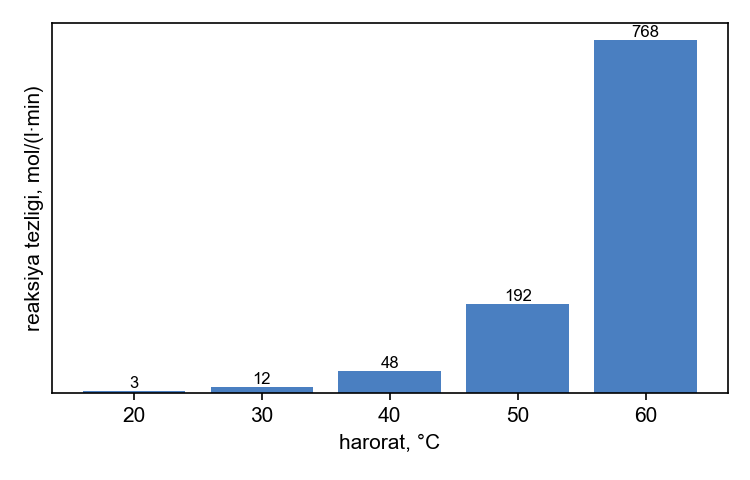
\includegraphics[width=0.86\linewidth]{rasmlar/gen/vh_v18_0.png}\end{center}
Reaksiyaning temperatura \textbf{koeffitsiyentini ($\gamma$) aniqlang.}

\noindent A)~\textsl{4} \hfill B)~\textsl{5} \hfill C)~\textsl{3} \hfill D)~\textsl{8}\par
\vspace{4pt}
\noindent\textbf{13.} K\textsubscript{2}CO\textsubscript{3} ning suvli eritmasi inert elektrodlar bilan elektroliz qilinganda qaysi moddalar ajraladi?

\noindent\begin{tabular}{@{}p{0.47\linewidth}@{}p{0.47\linewidth}@{}}
A)~\textsl{H\textsubscript{2} va O\textsubscript{2}} & B)~\textsl{Cu va Cl\textsubscript{2}} \\
C)~\textsl{Zn, H\textsubscript{2} va O\textsubscript{2}} & D)~\textsl{H\textsubscript{2}, Cl\textsubscript{2} va NaOH} \\
\end{tabular}\par
\vspace{4pt}
\noindent\textbf{14.} Qaysi juftliklar o`zaro reaksiyaga kirishmaydi? 1) Fe\textsubscript{2}O\textsubscript{3} va H\textsubscript{2}O; 2) SiO\textsubscript{2} va H\textsubscript{2}O; 3) Zn va NaOH; 4) NaCl va HNO\textsubscript{3}

\noindent A)~\textsl{3, 4} \hfill B)~\textsl{1, 4} \hfill C)~\textsl{1, 2, 4} \hfill D)~\textsl{1, 2, 3}\par
\vspace{4pt}
\noindent\textbf{15.} Cu + 4HNO\textsubscript{3} $\to$ Cu(NO\textsubscript{3})\textsubscript{2} + 2NO\textsubscript{2} + 2H\textsubscript{2}O jarayoni uchun tarkibida 50\% aralashma bo`lgan 128 g namuna (asosiy modda Cu) olingan. Cu(NO\textsubscript{3})\textsubscript{2} \textbf{massasini (g) aniqlang.}

\noindent A)~\textsl{376} \hfill B)~\textsl{94} \hfill C)~\textsl{282} \hfill D)~\textsl{188}\par
\vspace{4pt}
\noindent\textbf{16.} CO\textsubscript{2} + Ca(OH)\textsubscript{2} $\to$ CaCO\textsubscript{3} + H\textsubscript{2}O reaksiyasida 2,24 l (n.sh.) CO\textsubscript{2} ishtirok etdi. CaCO\textsubscript{3} \textbf{massasini (g) toping.}

\noindent A)~\textsl{20} \hfill B)~\textsl{10} \hfill C)~\textsl{5} \hfill D)~\textsl{15}\par
\vspace{4pt}
\noindent\textbf{17.} NaBr + AgNO\textsubscript{3} $\to$ AgBr + NaNO\textsubscript{3} reaksiyasida tarkibida 60\% aralashma bo`lgan 103 g namuna (asosiy modda NaBr) ishtirok etdi. AgBr \textbf{massasini (g) toping.}

\noindent A)~\textsl{150,4} \hfill B)~\textsl{37,6} \hfill C)~\textsl{112,8} \hfill D)~\textsl{75,2}\par
\vspace{4pt}
\noindent\textbf{18.} Ishqoriy metallar haqida qaysi fikrlar to`g`ri? 1) Kaliy suvdan og`ir; 2) KOH -- kuchli ishqor; 3) Ishqoriy metallar faqat oksidlovchi bo`ladi; 4) Natriy suv bilan reaksiyada H\textsubscript{2} va NaOH hosil qiladi

\noindent A)~\textsl{2, 3} \hfill B)~\textsl{2, 4} \hfill C)~\textsl{1} \hfill D)~\textsl{1, 2, 4}\par
\vspace{4pt}
\noindent\textbf{19.} Alyuminiy va magniy dan iborat 10,5 g aralashma mo`l NaOH eritmasida eritilganda 10,08 l (n.sh.) gaz ajraldi. Aralashmadagi magniy ning massa \textbf{ulushini (\%) aniqlang.}

\noindent A)~\textsl{77,1} \hfill B)~\textsl{22,9} \hfill C)~\textsl{11,4} \hfill D)~\textsl{69,4}\par
\vspace{4pt}
\noindent\textbf{20.} Rasmda aromatik uglevodorod hosilasining tuzilish formulasi berilgan.
\begin{center}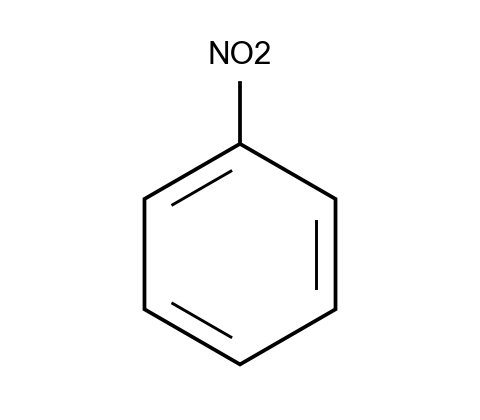
\includegraphics[width=0.86\linewidth]{rasmlar/gen/bz_770177.png}\end{center}
Molekuladagi $\sigma$-bog`lar \textbf{sonini aniqlang} ($\pi$-bog`lar halqada va o`rinbosarda alohida hisoblanadi).

\noindent A)~\textsl{14} \hfill B)~\textsl{15} \hfill C)~\textsl{13} \hfill D)~\textsl{16}\par
\vspace{4pt}
\noindent\textbf{21.} CH\textsubscript{3}--CH=C(CH\textsubscript{3})--CH\textsubscript{3} birikmaning sistematik nomi qaysi qatorda to`g`ri keltirilgan?

\noindent\begin{tabular}{@{}p{0.47\linewidth}@{}p{0.47\linewidth}@{}}
A)~\textsl{3-metilbuten-2} & B)~\textsl{2-metilbuten-3} \\
C)~\textsl{2-metilbuten-2} & D)~\textsl{2-metilbuten-1} \\
\end{tabular}\par
\vspace{4pt}
\noindent\textbf{22.} 15,6 g benzoldan nitrobenzol olishda unum 80\% bo`lsa, mahsulot \textbf{massasini (g) aniqlang} (boshlang`ich modda massasi 15,6 g).

\noindent A)~\textsl{19,68} \hfill B)~\textsl{24,6} \hfill C)~\textsl{39,36} \hfill D)~\textsl{12,48}\par
\vspace{4pt}
\noindent\textbf{23.} CH\textsubscript{3}OH va C\textsubscript{3}H\textsubscript{7}OH dan iborat 15,2 g aralashma natriy bilan to`liq reaksiyaga kirishganda 3,36 l (n.sh.) vodorod ajraldi. Aralashmadagi CH\textsubscript{3}OH \textbf{massasini (g) toping.}

\noindent A)~\textsl{12} \hfill B)~\textsl{6} \hfill C)~\textsl{15,2} \hfill D)~\textsl{3,2}\par
\vspace{4pt}
\noindent\textbf{24.} 22 g CH\textsubscript{3}CHO dan quyidagi ikki bosqichda CH\textsubscript{3}COOC\textsubscript{2}H\textsubscript{5} olinadi: 1) CH\textsubscript{3}CHO + 2Cu(OH)\textsubscript{2} $\to$ CH\textsubscript{3}COOH + Cu\textsubscript{2}O + 2H\textsubscript{2}O (unum 60\%); 2) CH\textsubscript{3}COOH + C\textsubscript{2}H\textsubscript{5}OH $\to$ CH\textsubscript{3}COOC\textsubscript{2}H\textsubscript{5} + H\textsubscript{2}O (unum 80\%). Oxirgi mahsulot CH\textsubscript{3}COOC\textsubscript{2}H\textsubscript{5} ning \textbf{massasini (g) toping.}

\noindent A)~\textsl{35,2} \hfill B)~\textsl{26,4} \hfill C)~\textsl{44} \hfill D)~\textsl{21,12}\par
\vspace{4pt}
\noindent\textbf{25.} Karbon kislotalar haqida qaysi fikrlar to`g`ri? 1) Sirka kislota karbonatlar bilan CO\textsubscript{2} ajratadi; 2) Sirka angidrid ikki molekula sirka kislotadan suv chiqib hosil bo`ladi; 3) Chumoli kislota "kumush ko`zgu" reaksiyasini beradi; 4) Karboksil guruh karbonil va gidroksil guruhlardan iborat

\noindent\begin{tabular}{@{}p{0.47\linewidth}@{}p{0.47\linewidth}@{}}
A)~\textsl{1, 3, 4} & B)~\textsl{1, 2, 3, 4} \\
C)~\textsl{1, 2, 4} & D)~\textsl{2, 3, 4} \\
\end{tabular}\par
\vspace{4pt}
\noindent\textbf{26.} 22 g C\textsubscript{2}H\textsubscript{5}COOCH\textsubscript{3} mo`l NaOH bilan to`liq gidrolizlandi. Hosil bo`lgan spirt \textbf{massasini (g) aniqlang.}

\noindent A)~\textsl{22} \hfill B)~\textsl{16} \hfill C)~\textsl{8} \hfill D)~\textsl{24}\par
\vspace{4pt}
\noindent\textbf{27.} Uglevodlar haqida qaysi fikrlar to`g`ri? 1) Selluloza $\beta$-glyukoza qoldiqlaridan iborat; 2) Glyukoza "kumush ko`zgu" reaksiyasini beradi; 3) Kraxmal yod bilan ko`k rang beradi; 4) Saxaroza Feling suyuqligini qaytaradi

\noindent A)~\textsl{1, 3} \hfill B)~\textsl{1, 2, 3} \hfill C)~\textsl{1, 2, 4} \hfill D)~\textsl{2, 3}\par
\vspace{4pt}
\noindent\textbf{28.} Aminlar, aminokislotalar va oqsillar haqida qaysi fikrlar to`g`ri? 1) Oqsillar biuret reaksiyasini beradi; 2) Aminokislotalar amfoter birikmalar; 3) Dipeptidda 2 ta peptid bog` bor; 4) Glitsin optik faol

\noindent A)~\textsl{1, 2} \hfill B)~\textsl{2, 3, 4} \hfill C)~\textsl{2, 3} \hfill D)~\textsl{4}\par
\vspace{4pt}
\noindent\textbf{29.} Reaksiya tenglamasi: C\textsubscript{2}H\textsubscript{4} + H\textsubscript{2} $\to$ C\textsubscript{2}H\textsubscript{6}. Reaksiyaga 22,4 l (n.sh.) C\textsubscript{2}H\textsubscript{4} kirishdi. C\textsubscript{2}H\textsubscript{6} \textbf{hajmini (l, n.sh.) hisoblang.}

\noindent A)~\textsl{44,8} \hfill B)~\textsl{22,4} \hfill C)~\textsl{11,2} \hfill D)~\textsl{33,6}\par
\vspace{4pt}
\noindent\textbf{30.} Metiloranj indikatori kislotali muhitda qanday rang beradi?
\noindent A)~\textsl{qizil}\par
\noindent B)~\textsl{malina rangga kiradi (pushti)}\par
\noindent C)~\textsl{rangsiz}\par
\noindent D)~\textsl{binafsha}\par
\vspace{4pt}
\noindent\textbf{31.} Rasmdagi asbobning elektrodlari quyidagi eritmalardan qaysi biriga tushirilganda lampochka yonadi?
\begin{center}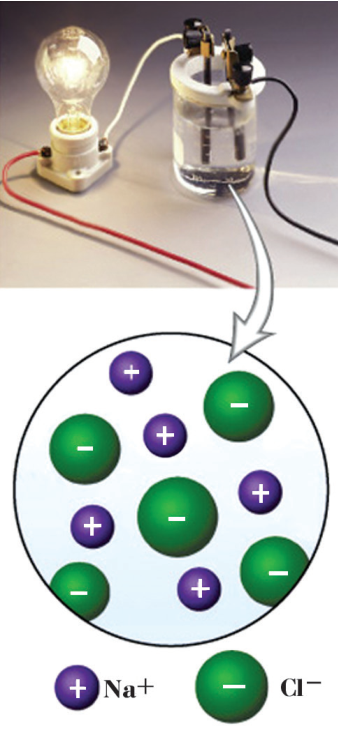
\includegraphics[width=0.86\linewidth]{rasmlar/darslik/d_elektr_asbob.png}\end{center}

\noindent\begin{tabular}{@{}p{0.47\linewidth}@{}p{0.47\linewidth}@{}}
A)~\textsl{distillangan suv} & B)~\textsl{mis sulfat eritmasi} \\
C)~\textsl{shakar eritmasi} & D)~\textsl{etanol} \\
\end{tabular}\par
\vspace{4pt}
\noindent\textbf{32.} Kimyo laboratoriyasida ishlash qoidalari haqida qaysi fikrlar to`g`ri? 1) Suvni konsentrlangan kislotaga tez quyish mumkin; 2) Ishqor teriga tushsa, qo`l suv bilan yuviladi; 3) Kimyoviy moddalar hidini bevosita nafas olib aniqlash kerak; 4) Spirt lampa boshqa lampadan yoqilmaydi

\noindent\begin{tabular}{@{}p{0.47\linewidth}@{}p{0.47\linewidth}@{}}
A)~\textsl{3} & B)~\textsl{1, 4} \\
C)~\textsl{2, 3, 4} & D)~\textsl{2, 4   ---} \\
\end{tabular}\par
\vspace{4pt}
\end{multicols}
\medskip
\noindent\setlength{\fboxsep}{0pt}\fbox{\begin{tabular}{p{0.74\linewidth}|p{0.2\linewidth}}
\parbox[t]{0.72\linewidth}{\vspace{3pt}\textbf{Topshiriqlar (33--35) va javob variant (A--F)larini o`zaro to`g`ri moslashtiring.} NaI va KBr dan iborat 26,9 g aralashma suvda eritilib, mo`l AgNO\textsubscript{3} eritmasi qo`shildi; hosil bo`lgan cho`kmalarning umumiy massasi 42,3 g.
\vspace{3pt}} & \parbox[t]{0.19\linewidth}{\vspace{3pt}A~\textsl{30}\\[3pt]
B~\textsl{18,6}\\[3pt]
C~\textsl{14,88}\\[3pt]
D~\textsl{15}\\[3pt]
E~\textsl{340}\\[3pt]
F~\textsl{22,5}}\\ \hline
\parbox[t]{0.72\linewidth}{\vspace{2pt}\textbf{33. Aralashmadagi NaI massasini (g) aniqlang.}\vspace{2pt}} & \\ \hline
\parbox[t]{0.72\linewidth}{\vspace{2pt}\textbf{34. Sarflangan 10\% li AgNO\textsubscript{3} eritmasining massasini (g) aniqlang (M(AgNO\textsubscript{3}) = 170 g/mol).}\vspace{2pt}} & \\ \hline
\parbox[t]{0.72\linewidth}{\vspace{2pt}\textbf{35. Eritmada hosil bo`lgan nitratlarning umumiy massasini (g) aniqlang.}\vspace{2pt}} & 
\end{tabular}}
\par\bigskip
\noindent\textbf{36.} KMnO\textsubscript{4} + Na\textsubscript{2}SO\textsubscript{3} + H\textsubscript{2}O $\to$ MnO\textsubscript{2} + Na\textsubscript{2}SO\textsubscript{4} + KOH reaksiya tenglamasini tenglang. Reagentlar (chap qism) koeffitsiyentlari \textbf{yig`indisini toping.}
\javob
\noindent\textbf{37.} 1 l hajmli yopiq idishda 1 mol N\textsubscript{2}O\textsubscript{4} qizdirilganda N\textsubscript{2}O\textsubscript{4} $\rightleftarrows$ 2NO\textsubscript{2} muvozanati qaror topdi. Muvozanat aralashmasining vodorodga nisbatan zichligi 38,33 ga teng. Shu haroratdagi muvozanat \textbf{konstantasini (K, mol/l) hisoblang.}
\javob
\noindent\textbf{38.} CaCO\textsubscript{3} va MgCO\textsubscript{3} dan iborat 26,8 g aralashma doimiy massagacha qizdirilganda qoldiq massasi 13,6 g bo`ldi. Aralashmadagi CaCO\textsubscript{3} ning \textbf{massasini (g) toping.}
\javob
\noindent\textbf{39.} C\textsubscript{3}H\textsubscript{7}OH va CH\textsubscript{3}OH dan iborat 9,2 g aralashma natriy bilan to`liq reaksiyaga kirishganda 2,24 l (n.sh.) vodorod ajraldi. Aralashmadagi C\textsubscript{3}H\textsubscript{7}OH \textbf{massasini (g) toping.}
\javob
\noindent\textbf{40.} 22,2 g propion kislota va 9,6 g metanol dan 75\% unum bilan murakkab efir olindi. Efir \textbf{massasini (g) toping.}
\javob
\par\bigskip\begin{center}\textbf{\fontsize{13}{15}\selectfont YOZMA ISH}\end{center}
\noindent\textbf{41.} \textbf{Topshiriqni bajarish jarayonida barcha reaksiya tenglamalarini yozing. Miqdoriy va arifmetik hisoblashlarni (unga asos bo`lgan usul yoki formulani ko`rsatgan holda) uzviy ketma-ketlikda bajaring.}\par\smallskip
Sulfat kislotaning massa ulushi 40\% bo`lgan eritmasining zichligi 1,3 g/ml.\par
\noindent 1)Eritmaning molyar konsentratsiyasini (mol/l) hisoblang.\par
\noindent 2)Eritmaning normal konsentratsiyasini (ekv/l) toping. Sulfat kislotaning ekvivalent massasini (g/ekv) ham aniqlang.\par
\noindent 3)Eritmaning molyal konsentratsiyasini (mol/kg) aniqlang.\par
\noindent 4)Shu eritmadan 250 ml 0,2 mol/l li eritma tayyorlash uchun necha ml olish kerak? 100 ml eritmadagi suvning massasini (g) ham hisoblang.\par
\noindent 5)100 ml shu eritmani to`liq neytrallash uchun necha gramm NaOH kerak? 250 ml shu eritmadagi H\textsubscript{2}SO\textsubscript{4} massasini (g) ham hisoblang.\par
\diqqat{Mazkur topshiriq kengaytirilgan javobni talab etib, uning yechilish usuli va shu usul asosidagi barcha hisoblash amallari javoblar varaqasida aks etishi lozim.}
\noindent\textbf{42.} Reaksiya tenglamalarini tugallang va tenglang. Hosil bo`lgan organik moddalarning tuzilish formulalarini yozing va ularni nomlang.\par
\noindent 1)n CH\textsubscript{2}=CH--CH=CH\textsubscript{2} $\to$\par
\noindent 2)CH\textsubscript{3}COONa + NaOH $\xrightarrow{\text{t}}$\par
\noindent 3)C\textsubscript{2}H\textsubscript{5}OH $\xrightarrow{\text{H\textsubscript{2}SO\textsubscript{4}(kons.), 170 \textdegree{}C}}$\par
\noindent 4)C\textsubscript{12}H\textsubscript{22}O\textsubscript{11} + H\textsubscript{2}O $\xrightarrow{\text{H\textsuperscript{+}}}$\par
\noindent 5)CH\textsubscript{3}CHO + Ag\textsubscript{2}O $\xrightarrow{\text{NH\textsubscript{3}, t}}$\par
\noindent 6)H\textsubscript{2}N--CH\textsubscript{2}--COOH + NaOH $\to$\par
\noindent 7)C\textsubscript{6}H\textsubscript{5}--CH\textsubscript{3} + Cl\textsubscript{2} $\xrightarrow{\text{yorug`lik}}$\par
\diqqat{Mazkur topshiriq kengaytirilgan javobni talab etib, uning yechilish usuli va shu usul asosidagi barcha hisoblash amallari javoblar varaqasida aks etishi lozim.}
\noindent\textbf{43.} \textbf{Topshiriqni bajarish jarayonida barcha reaksiya tenglamalarini yozing. Miqdoriy va arifmetik hisoblashlarni (unga asos bo`lgan usul yoki formulani ko`rsatgan holda) uzviy ketma-ketlikda bajaring.}\par\smallskip
120 g pirit (FeS\textsubscript{2}) yondirildi: 4FeS\textsubscript{2} + 11O\textsubscript{2} $\to$ 2Fe\textsubscript{2}O\textsubscript{3} + 8SO\textsubscript{2} (unum 80\%). Hosil bo`lgan SO\textsubscript{2} katalizator ishtirokida SO\textsubscript{3} gacha oksidlandi (unum 80\%), SO\textsubscript{3} suvda eritildi.\par
\noindent 1)Hosil bo`lgan SO\textsubscript{2} hajmini (l, n.sh.) va qattiq qoldiq Fe\textsubscript{2}O\textsubscript{3} massasini (g) hisoblang. Shuningdek SO\textsubscript{2} massasini (g) ham toping.\par
\noindent 2)SO\textsubscript{3} ning massasini (g) toping (2SO\textsubscript{2} + O\textsubscript{2} $\rightleftarrows$ 2SO\textsubscript{3}).\par
\noindent 3)Hosil bo`lgan H\textsubscript{2}SO\textsubscript{4} massasini (g) aniqlang.\par
\noindent 4)Shu kislotani to`liq neytrallash uchun zarur NaOH massasini (g) va mo`l BaCl\textsubscript{2} bilan hosil bo`ladigan cho`kma massasini (g) toping.\par
\noindent 5)Shu H\textsubscript{2}SO\textsubscript{4} dan 20\% li eritma tayyorlash uchun qancha suv (g) kerak?\par
\diqqat{Mazkur topshiriq kengaytirilgan javobni talab etib, uning yechilish usuli va shu usul asosidagi barcha hisoblash amallari javoblar varaqasida aks etishi lozim.}
\newpage
\noindent\textbf{\fontsize{13}{15}\selectfont Nazorat testi}\ \textit{$\cdot$ 18-variant}\hfill \textbf{Javoblar kaliti}\par\smallskip\hrule\smallskip
\textit{Faqat o`qituvchi uchun.}\par\medskip
\noindent\textbf{1--32-savollar}\par\smallskip
\noindent\begin{tabular}{|c|c|c|c|c|c|c|c|c|c|c|c|c|c|c|c|}\hline
\textbf{1} & \textbf{2} & \textbf{3} & \textbf{4} & \textbf{5} & \textbf{6} & \textbf{7} & \textbf{8} & \textbf{9} & \textbf{10} & \textbf{11} & \textbf{12} & \textbf{13} & \textbf{14} & \textbf{15} & \textbf{16}\\\hline
\textsl{C} & \textsl{C} & \textsl{C} & \textsl{A} & \textsl{B} & \textsl{D} & \textsl{A} & \textsl{D} & \textsl{C} & \textsl{D} & \textsl{C} & \textsl{A} & \textsl{A} & \textsl{C} & \textsl{D} & \textsl{B}\\\hline
\textbf{17} & \textbf{18} & \textbf{19} & \textbf{20} & \textbf{21} & \textbf{22} & \textbf{23} & \textbf{24} & \textbf{25} & \textbf{26} & \textbf{27} & \textbf{28} & \textbf{29} & \textbf{30} & \textbf{31} & \textbf{32}\\\hline
\textsl{D} & \textsl{B} & \textsl{B} & \textsl{A} & \textsl{C} & \textsl{A} & \textsl{D} & \textsl{D} & \textsl{B} & \textsl{C} & \textsl{B} & \textsl{A} & \textsl{B} & \textsl{A} & \textsl{B} & \textsl{D}\\\hline
\end{tabular}\par\medskip
\noindent\textbf{33--35-savollar}\par\smallskip
\noindent\begin{tabular}{|c|c|c|}\hline \textbf{No} & \textbf{Javob} & \textbf{Qiymat}\\\hline
33 & \textsl{D} & 15\\\hline
34 & \textsl{E} & 340\\\hline
35 & \textsl{B} & 18,6\\\hline
\end{tabular}\par\medskip
\noindent\textbf{36--40-savollar}\par\smallskip
\noindent\begin{tabular}{|c|c|}\hline \textbf{No} & \textbf{To`g`ri javob}\\\hline
36 & 6\\\hline
37 & 0,2\\\hline
38 & 10\\\hline
39 & 6\\\hline
40 & 19,8\\\hline
\end{tabular}\par\medskip
\noindent\textbf{41--43-topshiriqlar: qisqa yechim}\par\smallskip
\noindent\textbf{41-topshiriq.}\par
\noindent 1) C = 10$\cdot$$\omega$$\cdot$$\rho$/M = 10$\cdot$40$\cdot$1,3/98 = \textbf{5,306 mol/l}\par
\noindent 2) Cn = 2C = \textbf{10,612 ekv/l}; E = 98/2 = \textbf{49 g/ekv}\par
\noindent 3) 40 g H\textsubscript{2}SO\textsubscript{4} 60 g suvda: n = 0,408 mol $\to$ \textbf{6,803 mol/kg}\par
\noindent 4) \textit{V}\textsubscript{1} = C\textsubscript{2}\textit{V}\textsubscript{2}/C\textsubscript{1} = 0,2$\cdot$250/5,306 = \textbf{9,42 ml}; m(eritma) = 100$\cdot$1,3 = 130 g; suv = \textbf{78 g}\par
\noindent 5) n(H\textsubscript{2}SO\textsubscript{4}) = 5,306$\cdot$0,1 = 0,531 mol; NaOH = 2$\cdot$0,531$\cdot$40 = \textbf{42,45 g}; m = C$\cdot$\textit{V}$\cdot$M = 5,306$\cdot$0,25$\cdot$98 = \textbf{130 g}\par
\noindent Jami: M 15 + A 10 = 25 ball.\par
\noindent\textbf{42-topshiriq.}\par
\noindent 1) n CH\textsubscript{2}=CH--CH=CH\textsubscript{2} $\to$ (--CH\textsubscript{2}--CH=CH--CH\textsubscript{2}--)n --- polibutadiyen (3 ball)\par
\noindent 2) CH\textsubscript{3}COONa + NaOH $\xrightarrow{\text{t}}$ CH\textsubscript{4} + Na\textsubscript{2}CO\textsubscript{3} --- metan (4 ball)\par
\noindent 3) C\textsubscript{2}H\textsubscript{5}OH $\xrightarrow{\text{H\textsubscript{2}SO\textsubscript{4}(kons.), 170 \textdegree{}C}}$ CH\textsubscript{2}=CH\textsubscript{2} + H\textsubscript{2}O --- etilen (3 ball)\par
\noindent 4) C\textsubscript{12}H\textsubscript{22}O\textsubscript{11} + H\textsubscript{2}O $\xrightarrow{\text{H\textsuperscript{+}}}$ C\textsubscript{6}H\textsubscript{12}O\textsubscript{6} + C\textsubscript{6}H\textsubscript{12}O\textsubscript{6} --- glyukoza va fruktoza (4 ball)\par
\noindent 5) CH\textsubscript{3}CHO + Ag\textsubscript{2}O $\xrightarrow{\text{NH\textsubscript{3}, t}}$ CH\textsubscript{3}COOH + 2Ag$\downarrow$ --- etan (sirka) kislota (4 ball)\par
\noindent 6) H\textsubscript{2}N--CH\textsubscript{2}--COOH + NaOH $\to$ H\textsubscript{2}N--CH\textsubscript{2}--COONa + H\textsubscript{2}O --- glitsinning natriyli tuzi (3 ball)\par
\noindent 7) C\textsubscript{6}H\textsubscript{5}--CH\textsubscript{3} + Cl\textsubscript{2} $\xrightarrow{\text{yorug`lik}}$ C\textsubscript{6}H\textsubscript{5}CH\textsubscript{2}Cl + HCl --- benzilxlorid (4 ball)\par
\noindent Jami 25 ball.\par
\noindent\textbf{43-topshiriq.}\par
\noindent 1) n(FeS\textsubscript{2}) = 1 mol; SO\textsubscript{2}: 2n$\cdot$$\eta$ = 1,6 mol $\to$ \textbf{35,84 l}; Fe\textsubscript{2}O\textsubscript{3}: n/2$\cdot$$\eta$$\cdot$160 = \textbf{64 g}; m(SO\textsubscript{2}) = 1,6$\cdot$64 = \textbf{102,4 g}\par
\noindent 2) n(SO\textsubscript{3}) = 1,6$\cdot$0,8 = 1,28 mol $\to$ \textbf{102,4 g}\par
\noindent 3) SO\textsubscript{3} + H\textsubscript{2}O $\to$ H\textsubscript{2}SO\textsubscript{4}: \textbf{125,44 g}\par
\noindent 4) NaOH: 2$\cdot$1,28$\cdot$40 = \textbf{102,4 g}; BaSO\textsubscript{4}: 1,28$\cdot$233 = \textbf{298,24 g}\par
\noindent 5) m(eritma) = 125,44/0,2 = 627,2 g; suv = 627,2 $-$ 125,44 = \textbf{501,76 g}\par
\noindent Jami: M 15 + A 10 = 25 ball.\par
\par\bigskip\noindent\textbf{Mavzular taqsimoti}\par\smallskip
{\small\noindent\begin{longtable}{|c|p{7.2cm}|p{5.4cm}|c|}\hline \textbf{No} & \textbf{Mavzu} & \textbf{Tekshiriladigan ko`nikma} & \textbf{Ball}\\\hline
1 & Tirkashev VI bob (muvozanat, jadval) & Jadval tahlili & 1\\\hline
2 & 11-sinf 4-bob (molyal konsentratsiya) & Hisoblash va masala yechish & 1\\\hline
3 & 8-sinf; Tirkashev \textit{V} bob (oksidlanish darajasi) & Bilim va tushunish & 1\\\hline
4 & Tirkashev IV bob (kuchli elektrolitlar) & Hisoblash va masala yechish & 1\\\hline
5 & Tirkashev VI bob & Hisoblash va masala yechish & 1\\\hline
6 & Tirkashev III bob (eritmalar, jadval) & Jadval tahlili & 1\\\hline
7 & 11-sinf (gaz aralashmalar) & Hisoblash va masala yechish & 1\\\hline
8 & 11-sinf 4-bob (molyal konsentratsiya) & Hisoblash va masala yechish & 1\\\hline
9 & Tirkashev \textit{V} bob; 11-sinf 7-bob & Bilim va tushunish & 1\\\hline
10 & 10-sinf \S{}17 (gibridlanish); Abdusamatov & Bilim va tushunish & 1\\\hline
11 & 11-sinf (Mendeleyev--Klapeyron) & Hisoblash va masala yechish & 1\\\hline
12 & Tirkashev VI bob (Vant-Goff qoidasi, grafik) & Grafik tahlili & 1\\\hline
13 & 11-sinf 8-bob; Tirkashev \textit{V} bob (elektroliz) & Bilim va tushunish & 1\\\hline
14 & 9-sinf; Tashev (anorganik birikmalar xossalari) & Bilim va tushunish & 1\\\hline
15 & 9-sinf; Tirkashev (N/NH\textsubscript{3}/HNO\textsubscript{3}, hisob) & Hisoblash va masala yechish & 1\\\hline
16 & 9-sinf; Tirkashev (P/C/Si, hisob) & Hisoblash va masala yechish & 1\\\hline
17 & 9-sinf; Tirkashev (galogenlar, hisob) & Hisoblash va masala yechish & 1\\\hline
18 & 9-sinf (ishqoriy metallar); Tashev & Bilim va tushunish & 1\\\hline
19 & 9-sinf (alyuminiy) & Hisoblash va masala yechish & 1\\\hline
20 & 10-sinf (arenlar) & Rasm bo`yicha tahlil & 1\\\hline
21 & 10-sinf (nomenklatura \S{}6, \S{}11, \S{}20, \S{}24--26) & Bilim va tushunish & 1\\\hline
22 & 10-sinf \S{}16, \S{}23, \S{}33 & Hisoblash va masala yechish & 1\\\hline
23 & 10-sinf \S{}21 & Hisoblash va masala yechish & 1\\\hline
24 & 10-sinf (ikki bosqichli hisob) & Hisoblash va masala yechish & 1\\\hline
25 & 10-sinf (mavzuga oid paragraflar); Abdusamatov & Bilim va tushunish & 1\\\hline
26 & 10-sinf \S{}28 & Hisoblash va masala yechish & 1\\\hline
27 & 10-sinf (mavzuga oid paragraflar); Abdusamatov & Bilim va tushunish & 1\\\hline
28 & 10-sinf (mavzuga oid paragraflar); Abdusamatov & Bilim va tushunish & 1\\\hline
29 & 10-sinf (pol, hisob) & Hisoblash va masala yechish & 1\\\hline
30 & 8-sinf (indikatorlar) & Bilim va tushunish & 1\\\hline
31 & 9-sinf (elektrolitlar, 1-rasm) & Rasm bo`yicha tahlil & 1\\\hline
32 & 7-sinf (xavfsizlik qoidalari); 10-sinf lab. & Bilim va tushunish & 1\\\hline
33--35 & Aralash masala (moslashtirish) & Ko`p bosqichli hisob & 3\\\hline
36--40 & Qisqa javobli masalalar & Hisoblash & 5\\\hline
41--43 & Yozma ish & Usul va hisob (M, A) & 75\\\hline
\end{longtable}}
\end{document}
